\section{IQ Signal}
\subsection{Quadrature siganl}
    Quadrature signal은  복소수 체계를 기반으로 하기에 complex signal(복소 신호)라고도 불리며, I와 Q 2개로 이루어져 있으므로 I/Q 신호라고도 자주 불린다. Quadrature signal이 사용되는 신호처리를 quadrature processing이라고 한다.
    Quadrature signal은 특정 시간에서의 값을 하나의 복소수로 표현할 수 있는 2차원 신호"라고 수학적 으로 정의된다. 이때 각각을 실수부와 허수부를 in-phase와 quadrature phase라고 부르며 이 단어의 앞 글자를 따서 각각 $I$, $Q$라 한다.
    \begin{equation*}
        e^{jx} = I + Q
    \end{equation*}
    \vspace{-4mm}  
    \begin{figure}[!h]\centering
		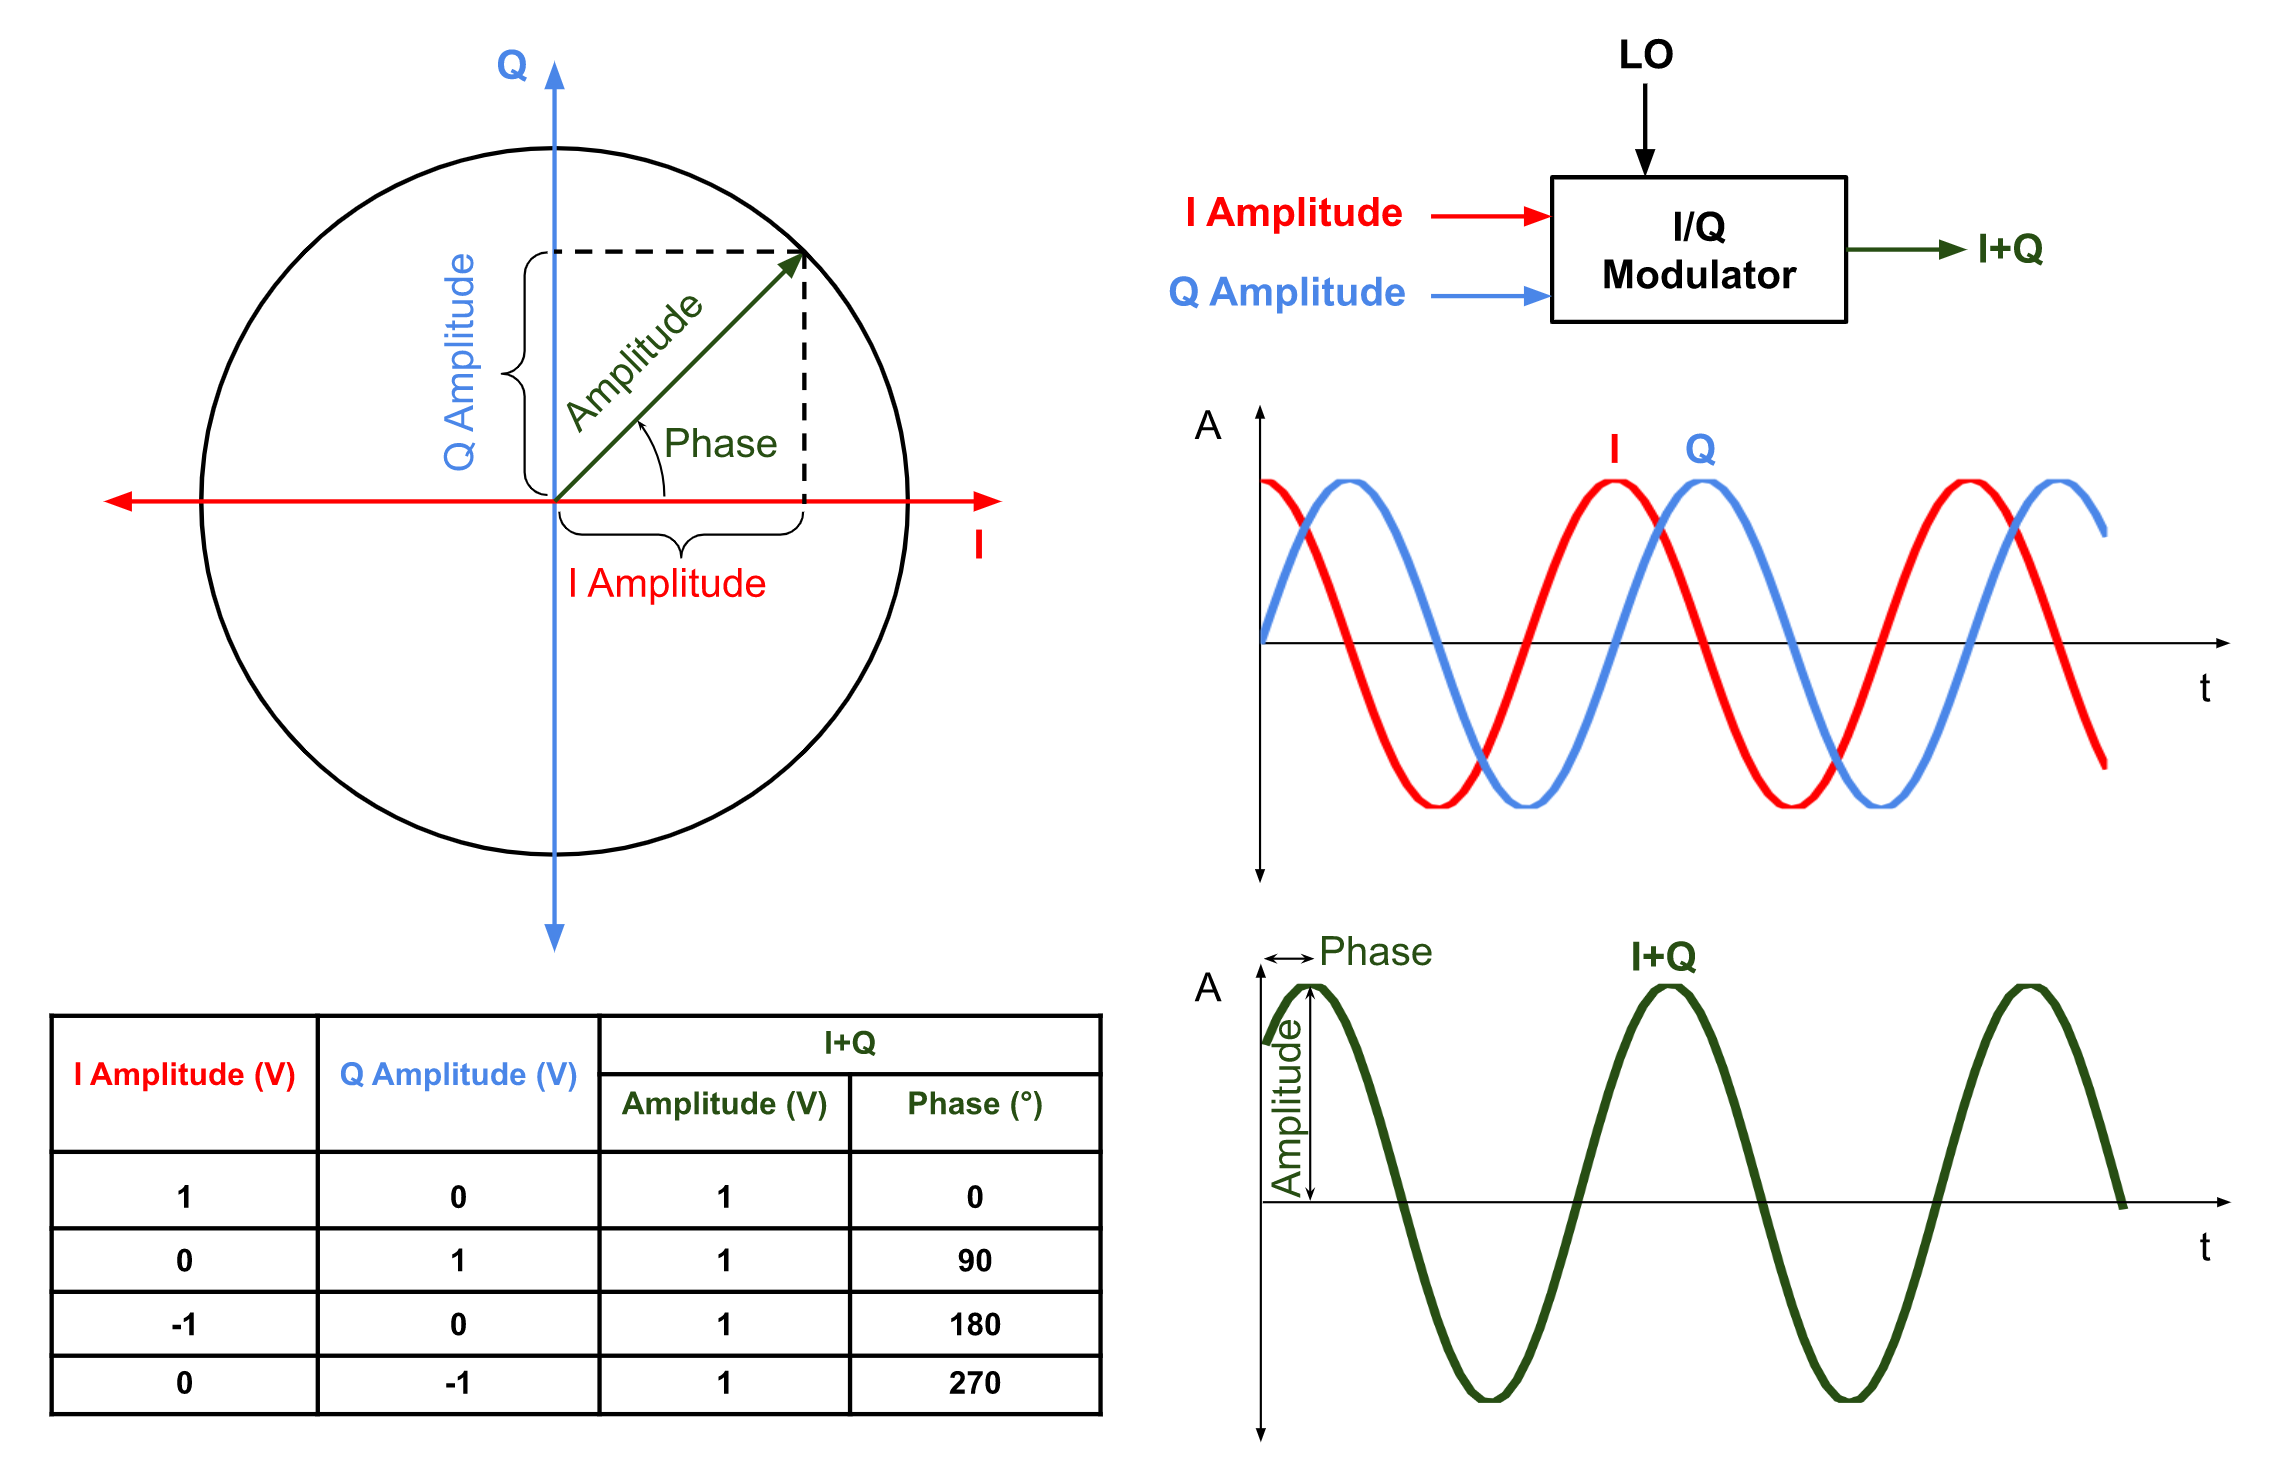
\includegraphics[width=.75\textwidth]{image/week02/2-0-1.png}
		\caption{\small IQ diagram}
		\vspace{-10pt}
    \end{figure}
\subsection{Quadrature Signal의 Time-Domain 에서 표현}
    Euler Equation으로 complex number를 표현할시에, magnitude $M = 1$이라하고, $\Phi = \omega t, \omega = 2 \pi f$로 하면 다음의 식을 얻을 수 있다. 
    \begin{equation*}
        c = e^{j2\pi f_0 t}
    \end{equation*}
    아래의 그림과 같이 복소수 c를 (a)의 점 또는 (b)의 벡터의 형태로 나타낼 수 있다. c는 (a)의 파란색 점과 같이 나타나는데, 시간 $t$가 증가하면 반시계 방향으로 이동한다. 주파수 $f$가 1일때 점은 1초에 1바퀴를 돌게된다. $f$ 대신 $-f$를 대입할 경우 음의 부호가 있는 하얀색 점과 같이 나타나는데, 파란색 점과 반대로 $t$가 증가하면 시계방향으로 이동한다.\\
\clearpage
    \vspace{-4mm}  
    \begin{figure}[!h]\centering
		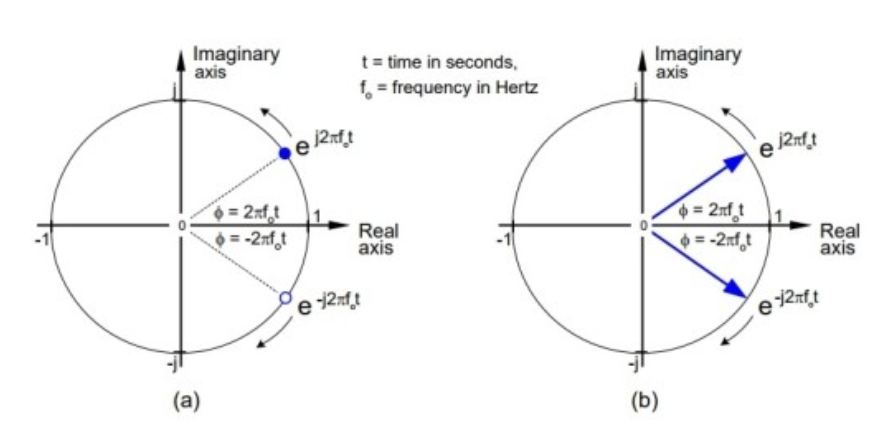
\includegraphics[width=.7\textwidth]{image/week02/2-1-1.png}
		\caption{\small Quadrature Signal Plot}
		\vspace{-10pt}
    \end{figure}
    위의 두가지 quadrature signal을 이용해 sine 함수와 cosine 함수를 유도할 수 있다. cosine 함수는 두 signal의 합, sine 함수는 두 signal의 차이다. 이를 응용하여 모든 quadrature signal은 sine, cosine 함수의 합으로 나타낼 수 있고 반대도 성립한다.\\
    \vspace{-6mm}
    \begin{align*}
        2\cos(2\pi f_0t) = e^{j2\pi f_0 t} + e^{-j2\pi f_0 t}\\
        2\sin(2\pi f_0t) = e^{j2\pi f_0 t} - e^{-j2\pi f_0 t}
    \end{align*}
    Quadrature signal은 2차원 신호이다. 여기에 시간이라는 축을 추가하면 다음과 같이 3차원 그래프로 나타낼 수 있다.\\
    
    \vspace{-4mm}  
    \begin{figure}[!h]\centering
		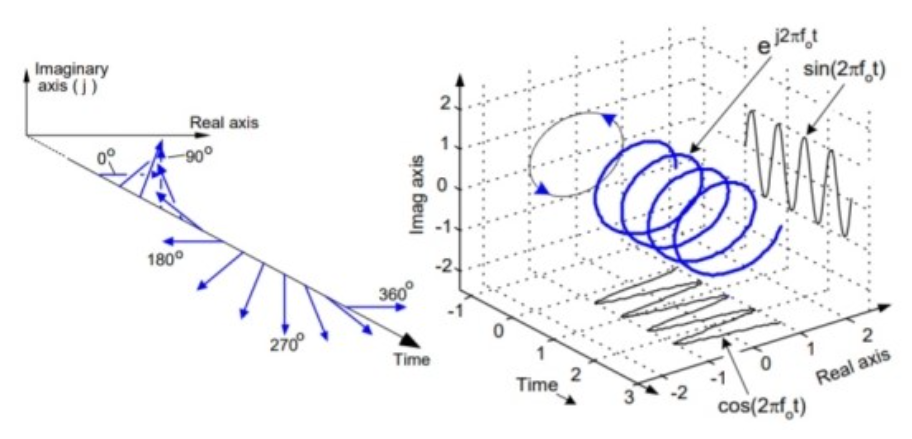
\includegraphics[width=.7\textwidth]{image/week02/2-1-2.png}
		\caption{\small Quadrature Signal in Time Domain}
		\vspace{-10pt}
    \end{figure}
    
    왼쪽의 figure는 시간에 따라 변하는 phasor를 vector로 표현한 것이고, 오른쪽 figure는 phasor의 시간에 따른 연속적인 변화를 표현한 것이다. 우측 figure에서 아래와 우측 평면에 cosine 함수와 sine 함수를 찾을 수 있는데 이 두 함수가 합쳐져 3차원 나선 모양의 quadrature signal을 만든 것이다.
\subsection{Quadrature Signal의 Frequency-Domain 에서 표현}
    \vspace{-4mm}  
    \begin{figure}[!h]\centering
		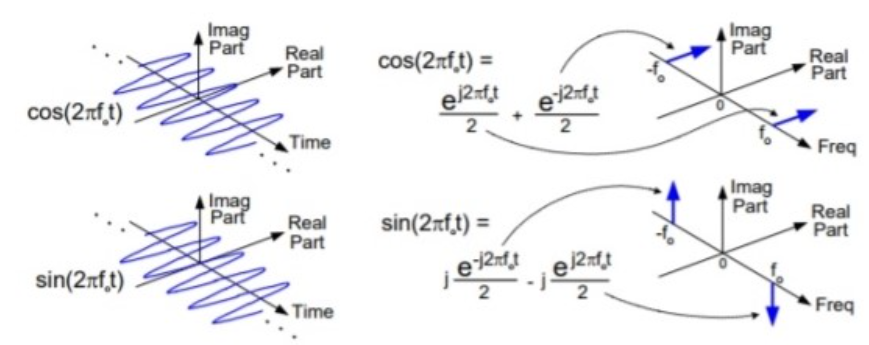
\includegraphics[width=.7\textwidth]{image/week02/2-2-1.png}
		\caption{\small Quadrature Signal in Time Domain and Frequency Domain}
		\vspace{-10pt}
    \end{figure}    
\clearpage
    이번에는 주파수 영역에서 quadrature signal의 성질을 확인해보자. 아래 그림은 복소평면에 각각 시간 축과 주파수 축을 추가한 것이다.
    시간 축으로 나타낸 좌측 그림에는 cosine 함수와 sine 함수가 허수 부분이 없이 실수로 나타나 있다. 우측 그림은 같은 cosine 함수와 sine 함수를 주파수 축에 나타낸 그림인데, 두개의 주파수 $f_0$ 과 $-f_0$에 impulse 형태로 표현된다. cosine 함수는 실수 축의 양의 방향으로 2개의 impulse가, sine 함수는 허수 축으로 양의 방향과 음의 방향 각각 1개의 impulse가 나타난다.이 두 함수를 응용하여 여러가지 quadrature signal을 만들 수 있다. \\
    \vspace{-4mm}  
    \begin{figure}[!h]\centering
		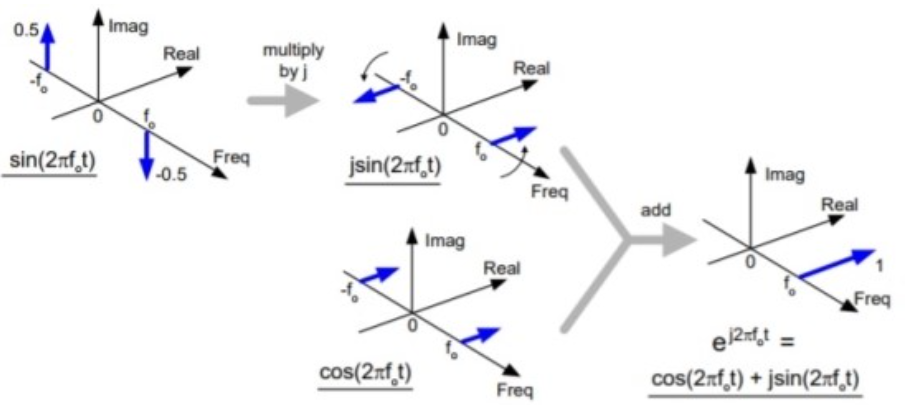
\includegraphics[width=.7\textwidth]{image/week02/2-2-2.png}
		\caption{\small Addition of two Quadrature Signals}
		\vspace{-10pt}
    \end{figure}
    
    다음의 그림과 같이 sine 함수에 j를 곱하여 반시계 방향으로 회전하여 실수 방향의 impulse를 만들 수 있다. 여기에 cosine 함수를 더하면 음의 방향의 impulse가 상쇄되어 하나의 impulse만 남게된다. 이는 Euler Equation에서 한가지 주파수 $f_0$을 갖는 것을 주파수 영역에 나타낸것과 동일하다.\\
    \vspace{-4mm}  
    \begin{figure}[!h]\centering
		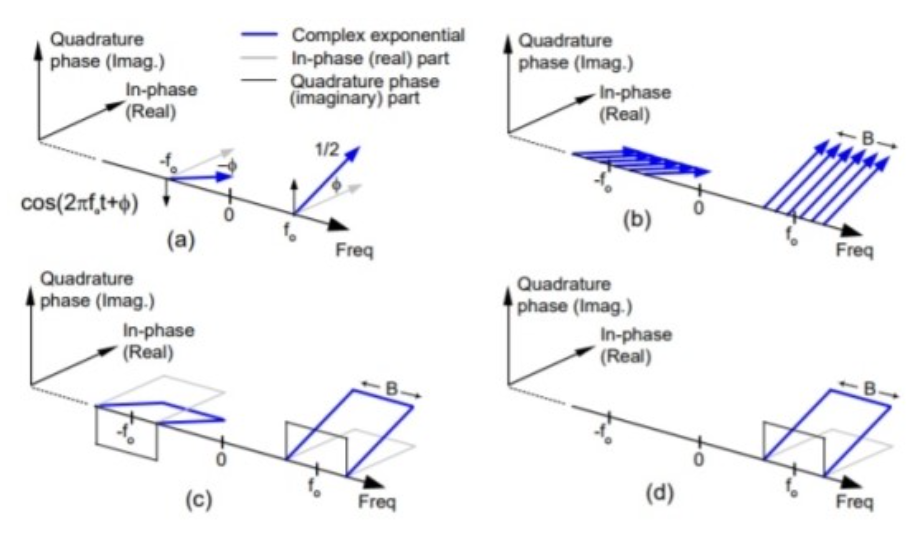
\includegraphics[width=.7\textwidth]{image/week02/2-2-3.png}
		\caption{\small Quadrature Signal with Phase}
		\vspace{-10pt}
    \end{figure}
    
    다음의 그림의 (a)는 cosine함수에 위상 $\phi$를 추가한 것을 주파수 영역에 나타낸 것이다. 원래 cosine 함수는 실수 성분만을 갖지만 위상 $\phi$가 추가됐을때 허수 성분이 추가되어 방향이 기울어지게 된다. 그림 (b), (c), (d)는 여러개의 phasor가 연속적으로 연결되어 대역대(bandwidth)를 이루는 신호들의 그림이다.\\
    \vspace{-4mm}  
    \begin{figure}[!h]\centering
		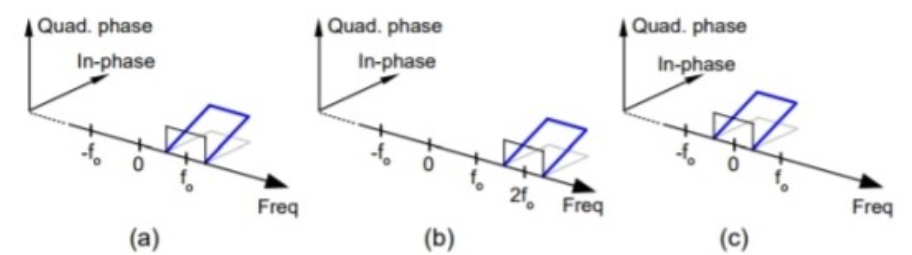
\includegraphics[width=.75\textwidth]{image/week02/2-2-4.png}
		\caption{\small Quadrature Mixing}
		\vspace{-10pt}
    \end{figure}


    
    주파수 대역을 바꾸는 것을 quadrature mixing 또는 complex mixing이라고 하는데 이를 주파수 영역에 나타내면 다음과 같다.
    (a)와 같이 주파수 $f_0$에 있는 신호에 $e^{j2\pi f_0 t}$를 곱하면 (b)와 같이 오른쪽으로 $f_0$만큼 이동한다. 반대로 $e^{-j2\pi f_0 t}$를 곱하면 (c)와 같이 왼쪽으로 $f_0$만큼 이동한다.\\

